\section{Construction, data and reproducibility}
\label{app:design}
\paragraph{Original papers.}
All six original-paper constructors used the requested and returned model identifier \texttt{gpt-6.1-sol}. Each had a fresh context and access to the task, the assigned article, supplementary search, the sampler contract and the generated-only inspection tool. The program, declared parameters and provenance notes were sealed before target comparison. The three final sampling seeds were 17121, 17123 and 17127. Each pressure draw had 3,000 rows and each iron draw 5,000. Estimators were also implemented independently using regression, counts and ranks. A target-family search preview in one pressure session contained survey identity, demographics and a qualitative topic. The session recorded and excluded it. The target slopes and paired correlation were withheld.

\paragraph{Pressure reference.}
The PNS operator uses the positive laboratory survey weight in a complete-case frame aged 20--79. It excludes recorded pregnancy. Unknown pregnancy status is retained under the frozen rule. The same rows enter both regressions. The design matrix contains an intercept, age, recorded sex and BMI in units of five kg/m$^2$. We correlate the residuals of the two pressure models. Synthetic records receive equal weights because the requested generator targets the weighted distribution. Five hundred row resamples retaining the survey weights gave conditional stability intervals of [2.96, 4.12] for the systolic slope, [1.93, 2.59] for the diastolic slope and [0.700, 0.734] for the residual correlation. The released workbook did not support a design-based cluster variance calculation.

\paragraph{Iron reference.}
NHANES August 2021--August 2023 supplies the measured hemoglobin, ferritin and survey-design variables. The eligible sample contains 979 nonpregnant women aged 20--44 with both measurements and positive phlebotomy weights. The frozen analysis uses raw ferritin with no inflammation adjustment. The three estimators are the weighted four-cell odds ratio, the weighted fraction with both markers low and a weighted Spearman correlation. A stratified delete-one-primary-sampling-unit calculation with 15 strata and 30 primary sampling units gave 95\% intervals of [9.28, 34.11] for the odds ratio, [6.07, 9.55]\% for both markers low and [0.318, 0.473] for the rank correlation.

\paragraph{Controlled evidence.}
The pressure and iron controls used nine fresh constructors each, with three seeded draws per constructor. The source block was masked before the modeling call. For pressure this hid or revealed six same-sample entries relating SBP, DBP, BMI and age. For iron it hid or revealed a paired contingency table. Neither experiment supplied the desired target result. The common base differed between cases, so cross-case comparisons of the base arm do not measure a shared zero-information condition. Both experiments used one model call per constructor, no feedback round and the same GPT identifier as the original-paper trials. Usage valued at the recorded tariffs was US\$0.92 for pressure and US\$0.68 for iron.

\paragraph{What orchestration adds.}
A separate developmental comparison started both an ordinary coding agent and a structured workflow from a research request. They had the same GPT model, search and runtime capabilities, and resource limits. Across 12 constructions and 36 seeded tables, the ordinary agent had smaller mean absolute discrepancies on four of the six focal analyses and the structured workflow on two. This result supports using a simple agent as a viable constructor. The source-to-code records serve the separate purpose of making each scientific choice inspectable.

\paragraph{Use of generative AI.}
The construction experiments used the model recorded above. OpenAI Codex also assisted in drafting the English manuscript, preparing the \LaTeX{} files and checking reported numerical results against the experimental artifacts.

\section{CHNS holdout, paired evaluation and local decomposition}
\label{app:chns}
\paragraph{Population.}
We linked 2,218 age-eligible women with the required survey fields. Of these, 2,205 had positive paired measurements. We converted the central Hb field from g/L to g/dL. Serum ferritin in ng/mL is numerically equal to $\mu$g/L. Ferritin was uncorrected for inflammation. Eligibility included all recorded pregnancy and inflammation statuses. We analyzed complete cases without national survey weights. Estimates describe this sample of women. Within province, a fixed hash ordering assigned alternate communities to A and B. We sealed the split, input hashes, research questions, tolerances and evidence schedule before model calls. The study articles supplied no measurements from B.

\paragraph{Construction.}
Each arm had three initial sessions. We interleaved the sessions and used the same GPT configuration and isolated runtime throughout. Each of the six parent programs had two sealed sibling revisions. One saw the original evidence and the source checks on the parent. The other also saw the added A contrast. All 18 requests returned programs. Each program drew 12,000 records at each of three common seeds. The scientific analysis pooled the three draws per program. The 54 tables are simulation repeats nested within six parents and one survey split. The 18 calls cost US\$1.77 at recorded token tariffs. A separate implementation reproduced the table analyses, the B intervals and both arm decisions before manuscript integration.

We computed Spearman correlation from average ranks for ties. For the crude odds ratio B had 114 both markers low, 116 only Hb low, 161 only ferritin low and 691 neither. The odds ratio is $(114\times691)/(116\times161)=4.218$. All four cells exceeded the minimum of ten. We used 2,000 province-stratified whole-community bootstrap replicates in each half. The B interval for correlation met the prespecified precision rule (half-width at most 0.10). The study's final-use rule required absolute rank error at most 0.10, an augmented odds ratio within a factor of 1.50 of B's, and augmented and control odds ratios within a factor of 1.20 of one another. All six passed. The primary incremental contrast subtracts augmented absolute rank error from control absolute rank error. A material arm-level benefit required all three pairs, median gain at least 0.05 with lower bootstrap limit above zero, at least two final-use passes and sufficient B precision. Conditional on the three parents per arm, the 95\% B-sampling intervals for the median gains were [$-0.0037$, $0.0037$] and [$-0.0035$, $0.0090$] for ordinary and guided sessions, respectively. Neither arm met the rule.

\begin{table*}[t]
\caption{All six CHNS sibling comparisons, with three pooled draws per program. C denotes revision with the original evidence. E denotes its sibling given the additional A contrast. A positive gain is a reduction in absolute error for the whole-cohort correlation. The final two columns describe errors in the probability-weighted middle-band contribution, examined after B was opened.}
\label{tab:chns}
\centering
\begin{tabular}{@{}lrrrrrr@{}}
\toprule
 & \multicolumn{4}{c}{Prespecified whole-cohort analyses} & \multicolumn{2}{c}{Exploratory local error}\\
\cmidrule(lr){2-5}\cmidrule(l){6-7}
Parent & Rank C & Rank E & Rank gain & Odds ratio E & C & E\\
\midrule
Ordinary 1 & 0.3003 & 0.2966 & $-0.0037$ & 5.1149 & 0.0034 & 0.0003\\
Ordinary 2 & 0.3078 & 0.3041 & $-0.0037$ & 4.9900 & 0.0081 & 0.0044\\
Ordinary 3 & 0.3176 & 0.3002 & $-0.0158$ & 5.1224 & 0.0172 & 0.0002\\
Guided 1 & 0.2927 & 0.3028 & $+0.0101$ & 5.0992 & 0.0104 & 0.0004\\
Guided 2 & 0.3075 & 0.3040 & $-0.0035$ & 5.1237 & 0.0109 & 0.0073\\
Guided 3 & 0.3201 & 0.2980 & $-0.0155$ & 4.9924 & 0.0230 & 0.0027\\
\bottomrule
\end{tabular}
\end{table*}

\paragraph{Exploratory covariance partition.}
Let $U,V$ denote global sample midranks of Hb and ferritin, each centered and standardized to unit variance with the full sample denominator. Let $G$ partition Hb at 12 and 14 g/dL. Then
\begin{align*}
\rho_S
  &= \operatorname{Cov}\{\mathbb E[U\mid G],\mathbb E[V\mid G]\}\\
  &\quad +\sum_g \Pr(G=g)\operatorname{Cov}(U,V\mid G=g).
\end{align*}
The middle-band value uses the original global ranks with the band-specific covariance and the band's sample weight. Reranking participants within the middle band would define a different statistic. In B, the between-band term was 0.270538 and the within-band terms were 0.011512, 0.034290 and 0.000460. Their sum gives 0.316800 up to rounding. For Guided 3 the middle contribution changed from 0.05726 to 0.03702 while the global rank correlation moved farther from B. Across parents, the between-band estimates were 0.2444--0.2489 with the original evidence and 0.2444--0.2474 with the extra contrast. Table~\ref{tab:chns} retains both the predeclared endpoints and the six descriptive component comparisons.

\subsection{A statistical model using the original CHNS evidence}
\label{app:chnsstat}
The retrospective comparator uses the same evidentiary inputs as the six original-evidence parents. The Zhu article supplies the scientific context and definitions. The A tables give numerical constraints in the survey population, so we use their counts and moments wherever the sources overlap. The model was specified after B was public. We recorded its equations, source hierarchy, scoring code, seeds and input hashes before scoring its draws. This compares statistical constructions given extracted evidence. It does not test article retrieval or extraction.

Let $G$ denote the three Hb bands. The model samples $G$ with probability $n_g/1123$. Conditional on $G$, it samples Hb and ferritin independently. For Hb we fit a beta distribution by moments on $(0,12)$ or $(12,14)$ and a shifted gamma law above 14. For $Y=\log(\mathrm{ferritin})$ we use the maximum-entropy density subject to the reported log mean, log variance and probability below $k=\log 15$. It has the form
\[
q_g(y)\ \propto\ \exp\{a_g y+b_g y^2+c_g\,\mathbf{1}_{y<k}\},\qquad b_g<0 .
\]
This is a normal density reweighted on either side of $k$. We set the two masses using the reported depletion frequency and solve for the underlying normal location and scale by matching the two log moments. At the resulting solution, every competing density satisfying the constraints has the same expectation of $\log q_g$. Nonnegativity of relative entropy then gives the stated entropy maximum on the log scale. This is one choice of marginal family and one assumption about dependence. Numerical integration verified all three fitted probabilities, means and dispersions against the A tables.

For the analytic population rank let $w_g=\Pr(G=g)$, $u_g=\sum_{j<g}w_j+w_g/2$, and $F_Y$ be the mixture CDF of log ferritin. Since the Hb bands are ordered and the two markers are independent within a band, $\rho_S=12\sum_g w_g u_g \mathbb E[F_Y(Y)\mid G=g]-3$. Integration gives 0.2414 and the four source cells give an OR of 5.083. The three 12,000-row draws gave ranks of 0.2456, 0.2451 and 0.2198. Pooling the records with the original estimator gives Table~\ref{tab:chnsattribution}. Direct per-draw rank and cell calculations reproduced both endpoints. The comparison uses zero additional model calls.

The re-pairing row uses the existing agent records. Under a random permutation of ferritin within each Hb band, the expected within-band covariance of the standardized global midranks is zero. All ranks and the number of threshold crossings per band retain their original marginal values. The between-band covariance in the preceding decomposition is therefore the exact expected Spearman correlation under that permutation. Table~\ref{tab:chnsattribution} reports its distance from B's estimate. The paired absolute-error reductions from the authored pairing ranged from 0.0454 to 0.0713. This is a conditional comparison on the six saved laws; the three seeds per law approximate that law's output.

\section{Every original-paper outcome}
\label{app:profiles}

\begin{figure*}[t]
\centering
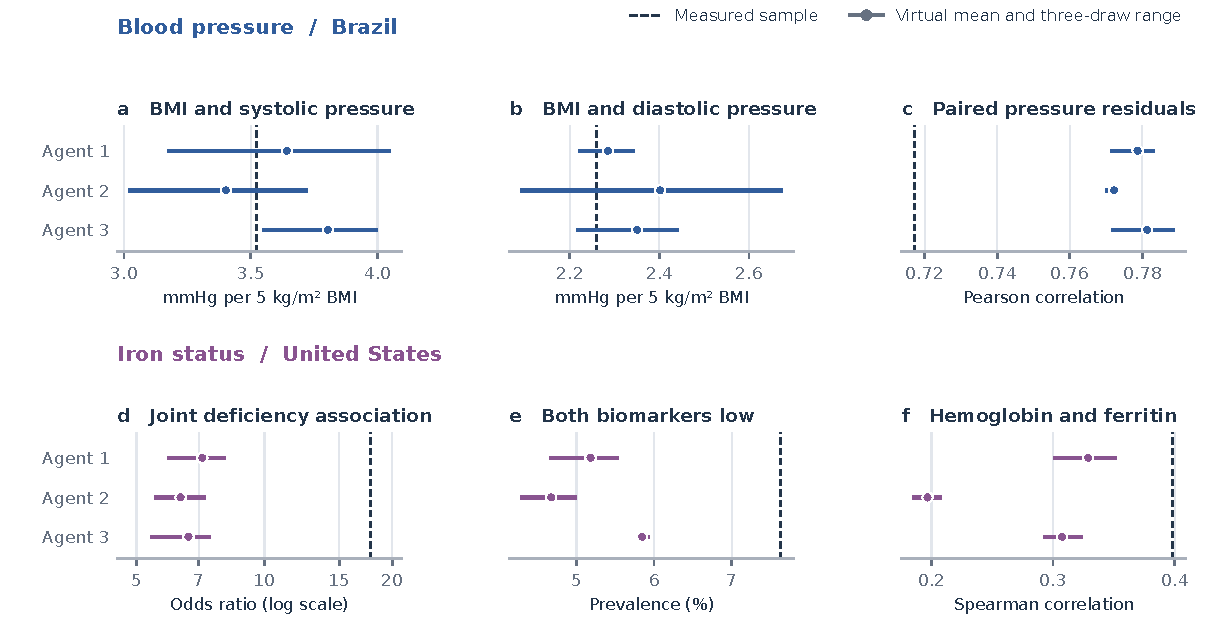
\includegraphics[width=.96\textwidth]{figures/original-paper.pdf}
\caption{The same analysis run on virtual and measured records. Each point is one constructor's mean across three seeded draws. The segment spans those draws. Dashed lines are measured sample estimates. Each panel has its own scale. The systolic slopes are near the Brazilian estimate. The iron odds ratios cluster around the value derived from the Chinese source paper, well below the US estimate.}
\Description{Six panels compare three constructors with a measured reference. The three systolic slopes straddle the reference, all diastolic slopes and residual correlations exceed it, and all three iron odds ratios, joint prevalences and rank correlations fall below their reference.}
\label{fig:original}
\end{figure*}

Table~\ref{tab:profile} preserves all three primary endpoints and the accompanying diagnostics in each case. Author numbers identify independent sessions within one task. The zero ordering violation rate follows from the positive pulse-pressure construction. Across the iron sessions, the two marginal deficiency fractions move in opposite directions relative to the US sample. The isolated threshold odds ratio is therefore an incomplete guide to biomedical utility.

\begin{table}[htbp]
\caption{All original-paper estimates. A1--A3 are constructor means over three seeded draws. The final column is the measured sample. Percentages use a 0--100 scale.}
\label{tab:profile}
\centering
\begin{tabular}{@{}lrrrr@{}}
\toprule
Analysis & A1 & A2 & A3 & Measured\\
\midrule
\multicolumn{5}{@{}l}{\emph{Brazilian blood pressure}}\\
BMI--SBP slope & 3.642 & 3.402 & 3.804 & 3.524\\
BMI--DBP slope & 2.285 & 2.402 & 2.350 & 2.260\\
Residual correlation & .779 & .772 & .781 & .717\\
SBP SD (mmHg) & 20.00 & 19.70 & 19.57 & 18.19\\
DBP SD (mmHg) & 11.57 & 11.57 & 11.47 & 11.09\\
SBP $<$ DBP (\%) & 0 & 0 & 0 & 0\\
\midrule
\multicolumn{5}{@{}l}{\emph{US iron status}}\\
Threshold odds ratio & 7.141 & 6.348 & 6.625 & 17.790\\
Both low (\%) & 5.180 & 4.673 & 5.847 & 7.630\\
Spearman correlation & .329 & .197 & .307 & .398\\
Low hemoglobin (\%) & 10.660 & 8.807 & 11.727 & 15.240\\
Low ferritin (\%) & 15.680 & 18.513 & 17.487 & 12.153\\
\bottomrule
\end{tabular}
\end{table}

\section{Two blood-pressure laws under the same constraints}
\label{app:laws}

\begin{figure*}[t]
\centering
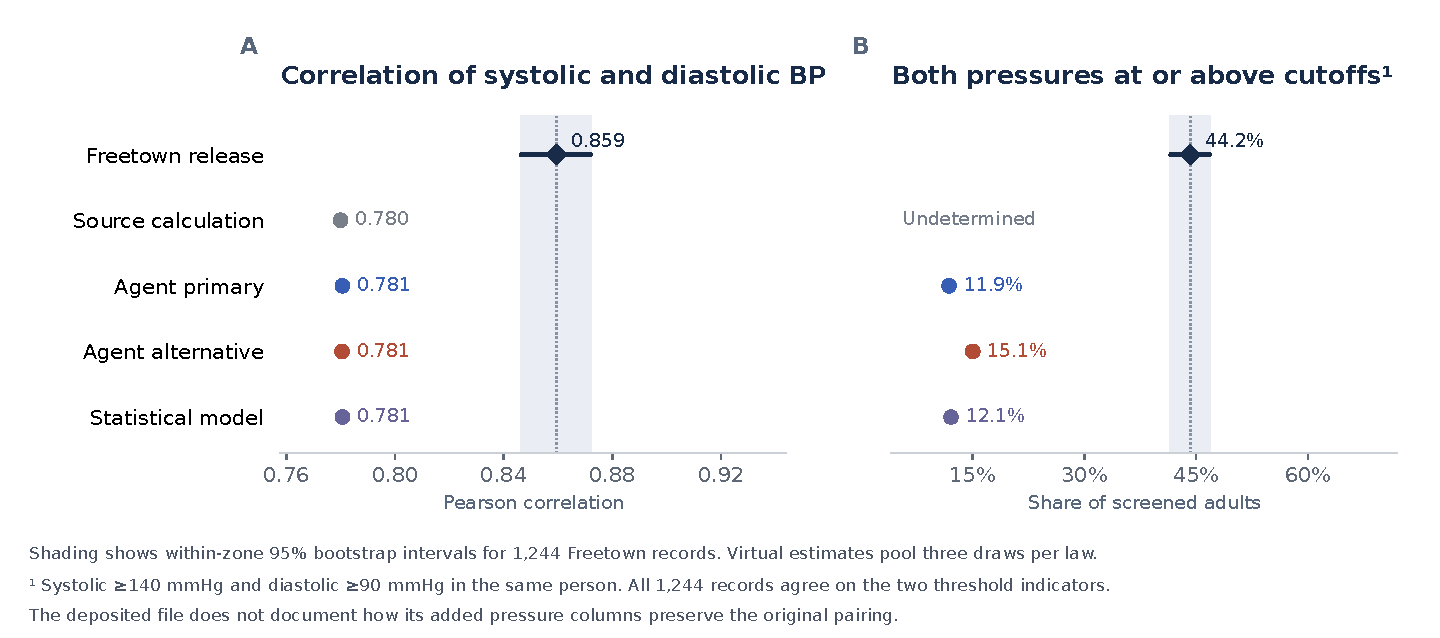
\includegraphics[width=.94\textwidth]{figures/freetown.pdf}
\caption{Prospective screening test. The source correlation is available by direct calculation. The joint threshold probability depends on the model. Points for the two agent laws and the statistical comparator are estimates from seeded virtual draws. The band describes uncertainty for the deposited Freetown sample conditional on the represented zones. The extreme target threshold result led to a separate audit of the deposited fields.}
\Description{Two panels show a released correlation of 0.859 and a joint threshold percentage of 44.2. Three virtual arms give correlations near 0.78 and threshold percentages between 11.9 and 15.1.}
\label{fig:freetown}
\end{figure*}

Let $S$ and $D$ be systolic and diastolic pressure. Write $G=S-D$ for the pulse-pressure gap. From the five source statistics, calculate
\begin{align*}
\mathrm{E}[G] &= \mathrm{E}[S]-\mathrm{E}[D],\\
\mathrm{Cov}(D,G) &= \mathrm{Cov}(S,D)-\mathrm{Var}(D),\\
\mathrm{Var}(G) &= \mathrm{Var}(S)+\mathrm{Var}(D)-2\mathrm{Cov}(S,D).
\end{align*}
The primary program draws positive $(D,G)$ from a bivariate lognormal distribution with these moments. For a vector of positive means $m$ and covariance $V$, the log covariance entries are $\log(1+V_{ij}/(m_i m_j))$ and the log means are $\log m_i$ minus half the corresponding log variance. Here the resulting matrices are positive definite. Setting $S=D+G$ enforces the intended ordering in every row.

The alternative program assigns probabilities 0.75 and 0.25 to components with means $(S,D)=(116.22,76.54)$ and $(152.22,92.54)$ mmHg. In $(D,G)$ coordinates, each component receives a common within-component covariance equal to the required total covariance minus the covariance of the component means. By the total covariance identity this gives the same unconditional first and second moments. The component probabilities and offsets are modeling choices. Conditional-normal quadrature for the event $\{D\geq90,\ D+G\geq140\}$ gives the probabilities in Section~\ref{sec:prospective}. Moments alone do not select either law.

\paragraph{Pre-disclosure design and measurement.}
The team screened eligibility, headers, uniqueness, measurement methods and field completeness before fixing the Freetown analysis. The target release identity and outcomes were withheld from the constructor. The primary, alternative, comparator, judgments and integration results were recorded before inspecting the measured joint outcomes. Construction took one recorded GPT call (US\$0.0845 at the recorded tariff). Each law generated three equal-sized draws of 10,000, including three for the independently implemented statistical comparator. The source protocol averaged the last two of three seated readings after at least 15 minutes' rest. Freetown averaged two readings following 3--5 minutes of rest. The source selected partnered rural adults, whereas the target was an urban community screening sample.

The Freetown reference uses paired positive recorded pressure values in prespecified age categories covering adults 40 and older. We computed an unweighted sample correlation and exceedance fraction. Intervals use 2,000 bootstraps of participants within eight zones, conditional on those zones. Across the full release, the audit counted 871 records meeting both thresholds, 1,523 meeting neither and zero in either discordant cell. These counts refer to deposited values. Field-level provenance would be needed to explain the pattern.



\section{Original-paper iron construction and verification}
\label{app:ironpros}

\begin{figure*}[t]
\centering
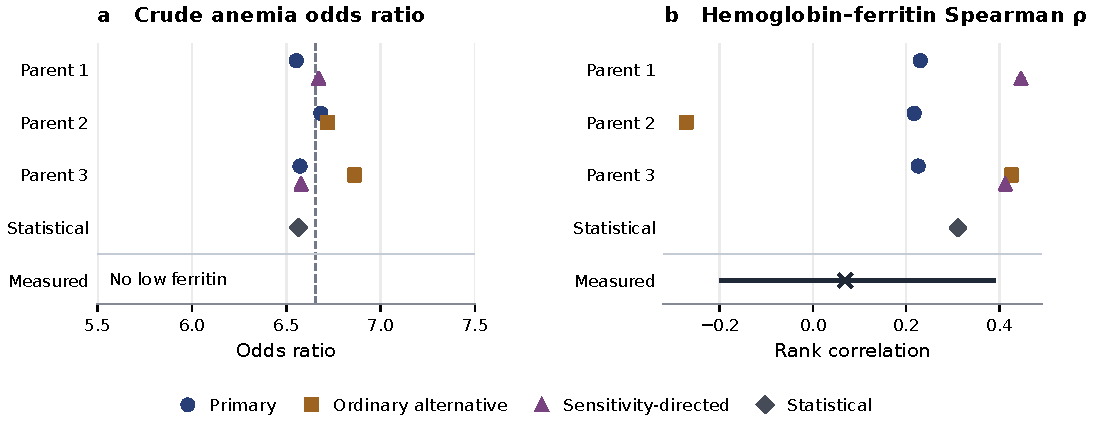
\includegraphics[width=.98\textwidth]{figures/iron-alternatives.pdf}
\caption{Two analyses on each sealed iron cohort. Symbols in each parent row distinguish the primary law and the two alternative requests. Two requests reached the output limit and have no point. The dashed line marks the source odds ratio of 6.65. The measured row gives the survey-weighted result for 44 women. The rank interval resamples villages within province. No woman in this sample had low measured ferritin.}
\Description{Agent odds ratios cluster between 6.55 and 6.86. Their rank correlations range from minus 0.272 to plus 0.446. The measured rank correlation is 0.069, with a wide interval.}
\label{fig:ironpros}
\end{figure*}

The protocol specified three independent primary sessions, two branches per primary, three seeds per executable law and 20,000 independent draws per seed. GPT-6.1 Sol received the original paper and a target description. It supplied the structure, parameters, prospective judgments and Python code. The statistical comparator used the same source and independent within-cell ranks. Two of nine requests (ordinary branch of parent 1, directed branch of parent 2) exhausted the 12,288-token output allowance. Usage across all nine requests cost an estimated US\$1.37 at the recorded tariff.

The original interface failed on all seven complete programs. Each program expected its named parameters at a different nesting level than the runner supplied. After the primary submissions were inspected and before simulated or measured outcomes were examined, we registered one mechanical rule to pass the nested parameter object following the same missing-key error on all three seeds. This rule preserved every scientific constant, line of sampler code, seed and target task. Original executions, failures and corrected executions were archived separately. The seven agent programs and one statistical program then produced 24 tables. All source assessments and model comparisons were committed before external disclosure.

The source checks cover four crude-cell frequencies, the crude log odds ratio, three hemoglobin-band frequencies, three ferritin-depletion fractions, three within-band ferritin geometric means, and both overall geometric means. These 16 checks overlap. Tolerances allow rounding, four estimated Monte Carlo standard errors and fixed operational allowances. Table~\ref{tab:ironprospective} gives the pooled simulated estimates. Each completed pair's absolute rank gap was 0.187--0.489. Subtracting its estimated 95\% Monte Carlo margin left 0.175--0.475. These margins describe simulation precision conditional on fixed laws.

\begin{table}[H]
\caption{Prospective iron analyses by parent and request. Each completed law contributes three draws. The last column records the complete source screen.}
\label{tab:ironprospective}
\centering
\begin{tabular}{@{}lrrl@{}}
\toprule
Construction & Odds ratio & Spearman $\rho$ & Screen\\
\midrule
P1 primary & 6.553 & 0.230 & pass\\
P1 ordinary & -- & -- & incomplete\\
P1 directed & 6.672 & 0.446 & pass\\
P2 primary & 6.683 & 0.217 & pass\\
P2 ordinary & 6.718 & -0.272 & pass\\
P2 directed & -- & -- & incomplete\\
P3 primary & 6.573 & 0.226 & pass\\
P3 ordinary & 6.862 & 0.426 & pass\\
P3 directed & 6.579 & 0.413 & pass\\
Statistical & 6.564 & 0.311 & pass\\
\bottomrule
\end{tabular}
\end{table}

\section{What can change while the selected iron summaries stay fixed?}
\label{app:ironproof}
Consider a single published hemoglobin band and ferritin-depletion cell with positive probability. Keep its probability and the two continuous conditional marginal distributions fixed. Draw hemoglobin from its conditional quantile function at a uniform rank $U$. One law draws ferritin from its conditional quantile at an independent uniform rank $V$. Another draws ferritin at $U$ with probability $\lambda>0$ and at $V$ otherwise. All other cells can stay fixed. The four threshold counts, each hemoglobin-band probability, and the ferritin geometric mean and depletion frequency in each band are invariant in the population. The overall geometric means are invariant as well.
For continuous marginal distributions, Spearman correlation is $12\,\mathbb{E}[F_H(H)F_F(F)]-3$. Within a nondegenerate cell the two marginal ranks are increasing functions of their corresponding uniforms. Sharing a uniform gives them positive covariance relative to independence. Hence the overall rank correlation changes while all the listed summaries remain fixed. This construction explains the ambiguity for the specified summaries. It supplies neither a biological estimate of the coupling nor its feasible range under additional evidence.

\section{Matched-size lifestyle analysis}
\label{app:lifestyle}

\begin{figure*}[t]
\centering
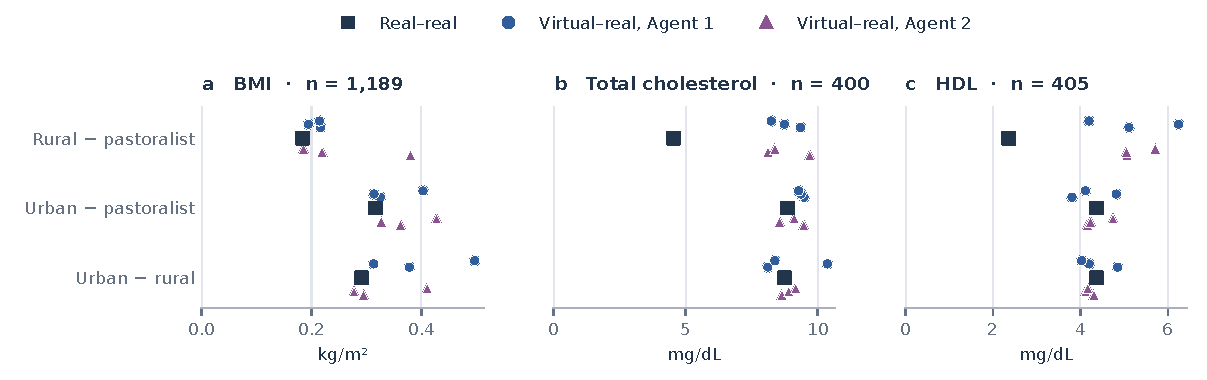
\includegraphics[width=.92\textwidth]{figures/lifestyle.pdf}
\caption{Matched-size mean absolute discrepancies for all nine adjusted lifestyle contrasts. The real--real estimate comes from two resamples of measured records. The virtual--real estimates use six saved virtual tables from two constructors. Native units and sample sizes differ across panels.}
\Description{Three panels compare BMI, total cholesterol and HDL across rural, urban and pastoralist lifestyles. Virtual versus real discrepancies are similar to real versus real for the urban BMI contrast, and larger for both rural lipid contrasts.}
\label{fig:lifestyle}
\end{figure*}

The original Turkana regression compared three lifestyle groups, adjusting each trait for age and sex~\cite{lea}. Real and virtual samples were matched on six sex-by-lifestyle stratum sizes within each trait. There were 1,189 eligible BMI measurements, 400 total cholesterol measurements and 405 HDL measurements. Each of 500 repetitions drew two real samples from the same empirical pool and one sample from each fixed virtual table. The virtual samples shared the second real sample as their reference. This design conditions on sample size, available cases and stratum counts. It leaves age and the outcomes free to vary. The bootstrap uses participants and does not model household or site clustering.



\begin{table*}[t]
\caption{Absolute discrepancies in matched-size lifestyle regressions. R and U denote rural and urban groups, and P denotes pastoralists. V--R gives the range across six fixed tables.}
\label{tab:lifestyle}
\centering
\begin{tabular}{@{}llrr@{}}
\toprule
Outcome & Contrast & Real--real & V--R\\
\midrule
BMI & R--P & .184 & .185--.380\\
(kg/m$^2$) & U--P & .316 & .314--.428\\
 & U--R & .291 & .277--.497\\
\midrule
Total cholesterol & R--P & 4.543 & 8.118--9.695\\
(mg/dL) & U--P & 8.848 & 8.556--9.479\\
 & U--R & 8.743 & 8.110--10.365\\
\midrule
HDL cholesterol & R--P & 2.363 & 4.195--6.242\\
(mg/dL) & U--P & 4.375 & 3.807--4.818\\
 & U--R & 4.362 & 4.029--4.851\\
\bottomrule
\end{tabular}
\end{table*}

Only 37 urban participants contributed total cholesterol measurements and 38 contributed HDL measurements. This small group helps explain the wide real--real variation. The discrepancy estimates in Table~\ref{tab:lifestyle} describe the observed composition. Equivalence for a planning decision would require a tolerance justified for that decision.
